\pdfpagewidth=8.5in 
\pdfpageheight=11in


\documentclass{sig-alternate}
\usepackage[utf8]{inputenc} 
\usepackage[T1]{fontenc}
\usepackage{microtype}

\usepackage{url}
\usepackage{amsmath}
\usepackage{graphicx}
\usepackage{subfigure}
\usepackage{threeparttable}
\usepackage{pdflscape}
\usepackage{array}
\usepackage{color}

\usepackage{flushend}

\begin{document}

\conferenceinfo{MSR}{'14, May 31 – June 1, 2014, Hyderabad, India}
\CopyrightYear{2014}
\crdata{978-1-4503-2863-0/14/05}

\title{The Bug Catalog of the Maven Ecosystem}

\numberofauthors{1}

%\author{
%% 1st. author
%\alignauthor
%Dimitris Mitropoulos\\
%       \affaddr{Athens University of Economics and Business}\\
%       \affaddr{Department of Management Science and Technology}\\
%       \email{dimitro@aueb.gr}
%% 2nd. author
%\alignauthor Vassilios Karakoidas\\
%       \affaddr{Athens University of Economics and Business}\\
%       \affaddr{Department of Management Science and Technology}\\
%       \email{bkarak@aueb.gr}
%% 3rd. author
%\alignauthor Panos Louridas\\
%       \affaddr{Athens University of Economics and Business}\\
%       \affaddr{Department of Management Science and Technology}\\
%       \email{louridas@aueb.gr}
%\and  % use '\and' if you need 'another row' of author names
%% 4th. author
%\alignauthor Georgios Gousios\\
%       \affaddr{Delft University of Technology}\\
%       \affaddr{Software Engineering Research Group}\\
%       \email{G.Gousios@tudelft.nl}
%% 5th. author
%\alignauthor Diomidis Spinellis\\
%       \affaddr{Athens University of Economics and Business}\\
%       \affaddr{Department of Management Science and Technology}\\
%       \email{dds@aueb.gr}
%}

\def\aueb{\textsuperscript{*}}
\def\tud{\textsuperscript{\dag}}

\author{
  Dimitris Mitropoulos\aueb \and Vassilios Karakoidas\aueb \and Panos Louridas\aueb \and Georgios Gousios\tud \and Diomidis Spinellis\aueb \\
  \begin{tabular}{ccc}
  \affaddr{\aueb Department of Management Science and Technology} & & \affaddr{\tud Software Engineering Research Group}\\
    \affaddr{\aueb Athens University of Economics and Business} & & \affaddr{\tud Delft University of Technology}\\
   \affaddr{Athens, Greece} & & \affaddr{Delft, the Netherlands}\\
   \email{\{dimitro,bkarak,louridas,dds\}@aueb.gr}& & \email{g.gousios@tudelft.nl} \\
  \end{tabular}
}

\maketitle
\begin{abstract}
Examining software ecosystems can provide the research community
with data regarding artifacts, processes, and communities.
We present a dataset obtained from the Maven central repository
ecosystem (approximately 265{\sc gb} of data) by statically analyzing
the repository to detect potential software bugs.
For our analysis we used {\it FindBugs}, a tool that examines Java
bytecode to detect numerous types of bugs.
The dataset contains the metrics results that FindBugs reports for
every project version (a {\sc jar}) included in the ecosystem. For every
version we also stored specific metadata such as the {\sc jar}'s
size, its dependencies and others. Our dataset can be used to produce
interesting research results, as we show in specific examples.
\end{abstract}

\category{D.2.4}{Software Engineering}{Software/Program Verification}[Statistical methods]
\category{D.2.5}{Software Engineering}{Testing and Debugging}[Code inspections and walk-throughs]
\category{D.2.7}{Software Engineering}{Distribution, Maintenance, and Enhancement}[Version control]

\terms{Static Analysis, Software Ecosystems.}

\keywords{Maven Repository, FindBugs, Software Bugs.}

\section{Introduction}
\label{sec:intro}

A software ecosystem can be seen as a collection of software projects,
which are developed and co-evolve in the same environment~\cite{LL10}.
Components can be interdependent and have multiple versions.
Examples of such ecosystems include Python's
{\sc p}y{\sc py}\footnote{\small \url{http://pypy.org/}}
(Python Package Index), Perl's
{\sc cpan}\footnote{\small \url{http://www.cpan.org/}}
(Comprehensive Perl Archive Network), Ruby's
RubyGems\footnote{\small \url{http://rubygems.org/}}
and the Maven Central Repository.\footnote{\small \url{http://mvnrepository.com/}}

Maven is a build automation tool used primarily for Java projects and it is
hosted by the Apache Software Foundation.\footnote{\small \url{http://maven.apache.org/}}
It uses {\sc xml} to describe the software project being built, its dependencies
on other external modules, the build order, and required plug-ins.
To build a software component, it dynamically downloads Java libraries
and Maven plug-ins from the {\it Maven central
repository},\footnote{\small \url{http://mvnrepository.com/}}
and stores them in a local cache. The repository can be updated with
new projects and also with new versions of existing projects
that can depend on other versions.

To statically analyze the Maven repository
we used {\it FindBugs},\footnote{\small \url{http://findbugs.sourceforge.net/}}
a static analysis tool that examines bytecode to detect software bugs
and has already been used in research~\cite{AP10,SHP06}.
Specifically, we ran FindBugs on all the project versions of all
the projects that exist in the repository
to identify all bugs contained in it.

In this paper we present: a) the construction process to obtain the
collection of the metrics results that the FindBugs tool produces 
for every project version of the repository (115,214 {\sc jar}s),
b) our dataset
and c) how researchers can use the dataset and produce
meaningful results.

\begin{table}
\centering
\scalebox{0.94}{
\begin{tabular}{l r}
\hline
Measurement & Value\\
 \hline
Projects & 17,505\\
Versions (total) & 115,214\\
Min (versions per project) & 1\\
Max (versions per project) & 338\\
Mean (versions per project) & 6.58\\
Median (versions per project) & 3\\
Range (over versions) & 337\\
1$^{st}$ Quartile (over versions) & 1\\
3$^{rd}$ Quartile (over versions) & 8\\
\hline
\end{tabular}
}
\caption{Descriptive statistics measurements for the Maven repository.}
\label{tbl:repository}
\end{table}

\section{Dataset Construction Process}
\label{sec:exp}

The dataset construction consisted of two basic steps,
namely: {\it data cleaning} and {\it FindBugs results
collection}. Table~\ref{tbl:tools-size} presents some
metrics concerning the tools created for
the process.

\begin{table}
\centering
\begin{tabular}{l r}
 \hline
\verb|Python Scripts| & 14\\
\verb|Lines of Code| & 1256\\
\verb|Code Size (KB)| & 92\\
\hline
\end{tabular}
\caption{Size metrics concerning
the tools created for
the dataset construction process.}
\label{tbl:tools-size}
\end{table}

{\bf Data Cleaning} Initially, we obtained a snapshot
(January 2012) of the Maven repository and handled it
locally to retrieve a list
of all the names of the project versions that existed in
it. In addition, we filtered out projects written in programming
languages other than Java (such as Scala, Groovy, Clojure, etc.)
because FindBugs analyzes only Java bytecode.
Since our construction process took place at the end of 2012,
several versions were released for some of the projects.
Thus, we cross-checked
the local versions with those online\footnote{\small \url{http://mirrors.ibiblio.org/maven2/}}
and supplemented the missing {\sc jar}s that have been
added to the repository during this period.
The statistic measurements concerning
the repository can be seen in Table~\ref{tbl:repository}
and the distribution of version
count among the selected projects is
presented in Figure~\ref{fig:version-count}.

\begin{figure}[t]
	\centering
	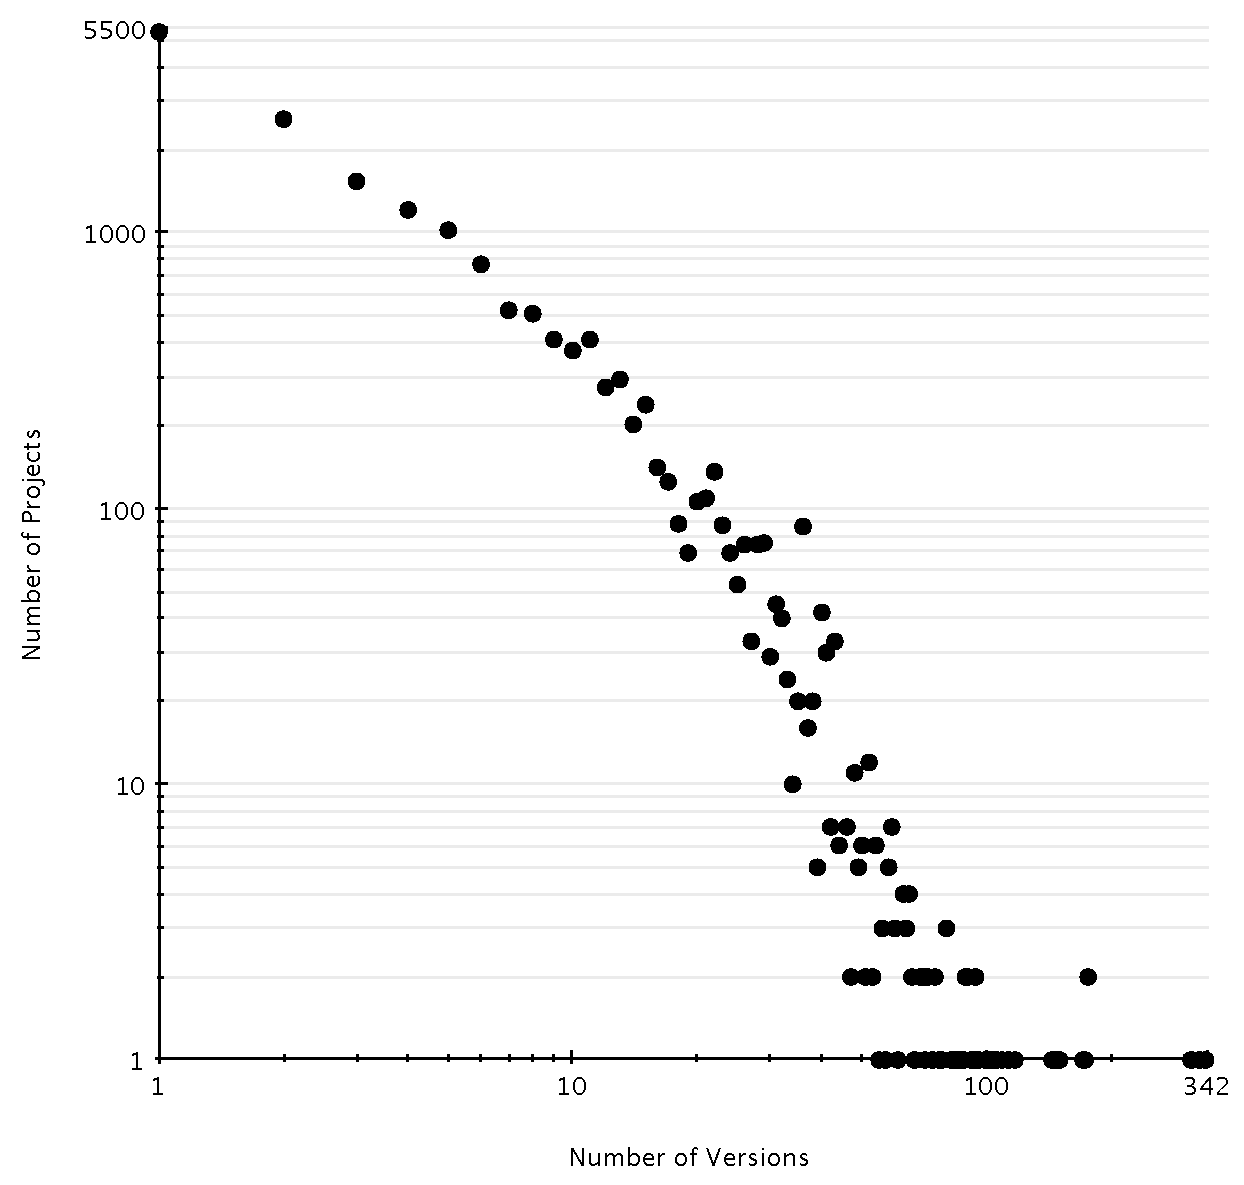
\includegraphics[scale=0.37]{version_count.pdf}
	\caption{Distribution of version count among project population.}
	\label{fig:version-count}
\end{figure}

%The first is to filter out non-Java jars... for that we used the following heuristics: 

%- heuristic 1
%- heuristic 2 

%The data collection process started with the mirroring of the Maven repository.
%The repository typically contains the {\sc jar} files with sources and binary distributions, 
%{\sc xml} metadata files that contain the version list for each project and its dependencies and one 
%metadata file, also in {\sc xml} format, with specific data for each version.

%We exported a list of all the {\sc jar} files in the repository and initially we excluded those
%that contained the source distribution for the projects. Then we kept all those {\sc jar}s that 
%referred to Java projects, because Findbugs analyzes only applications written in Java,
%and the Maven repository hosts projects from languages other than Java such as Scala, Groovy,
%Clojure, etc. 

%The initial snapshot of the repository was obtained in January 2012 and those experinment took
%place in the end of 2012. The statistic measurements concerning the repository can be seen in 
%Table~\ref{tbl:repository}. In the meantime, several versions were released for some of the selected project.
%We added them in an incremental way, using the following methodology; we implemented a script that cross-checked 
%all the local versions of the project with those online;\footnote{\url{http://mirrors.ibiblio.org/maven2/}} and downloaded
%the missing ones.

{\bf FindBugs Results Collection} The dataset
size prohibited the analysis
on a single host. For this reason,
we opted for distributed processing.
A schematic representation of the collection of
the FindBugs metrics results can be seen in Figure~\ref{fig:arch}.

%We created an architecture that can be seen in Fig (add figure).
%Jobs were put into the queue, results in Mongo.... It took 29 (?)
%hours, that many records were produced that many records failed
%because of reasons 12,,3 etc

In particular, we created a series of processing tasks
based on the {\sc jar} list from the
previous step, and added them to a task queue mechanism (a
Rabbit{\sc mq} message broker). Then we executed twenty five
workers (custom Python scripts) that checked out tasks from
the queue, processed each project version and stored the
results to the data repository (a Mongo{\sc db} database system).
The collection process lasted for approximately four and
a half days.

\begin{figure}[t]
  \begin{center}
    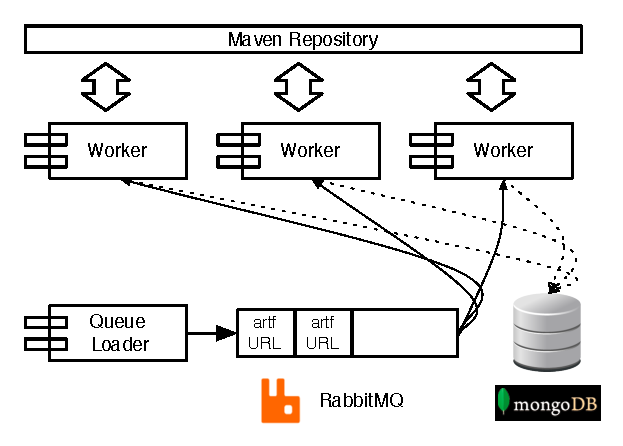
\includegraphics[scale=0.66]{figures/arch.pdf}
  \end{center}
  \caption{The data processing architecture.}
  \label{fig:arch}
\end{figure}

A typical processing cycle of a worker included the
following steps: after the worker spawned, it requested a task
from the queue. This task contained the {\sc jar} name, which
was typically a project version that was downloaded locally.
First, specific {\sc jar} metadata were calculated and stored
(see Section~\ref{sec:data}).
Then, FindBugs was invoked
by the worker and its results were also stored in the data
repository.
Note that before invoking FindBugs,
the worker checked if the {\sc jar} is valid in terms of implementation.
For instance, for every {\sc jar} the worker checked
if there were any {\it .class} files before invoking FindBugs.
When the task was completed
the queue was notified and the next task was requested.

When the data collection was completed, we ran some tests
to check the validity of the results.
A common issue that we discovered was the out-of-memory
crashes of Findbugs, which demanded the repetition of the process
for the corresponding {\sc jar}s, with the appropriate
settings in the Java Runtime Environment ({\sc jre}).
%The sanitisation process was consisted of four iterations,
%until all our scripts indicate that our data was correct. 

\section{Dataset Contents}
\label{sec:data}

\begin{table}[t]
\centering
\scalebox{0.78}{
\begin{tabular}{l p{16em}}
\hline
Category & Description\\
\hline
Bad Practice & Violations of recommended and essential
coding practice. \\
Correctness & Involves coding misting a way that is particularly different from the other bug sakes resulting in code
that was probably not what the developer intended. \\
Experimental & Includes unsatisfied obligations. For instance,
forgetting to close a file. \\
Internationalization (i18n) & Indicates the use of non-localized methods. \\
Multi-Threaded ({\sc mt}) Correctness & Thread synchronization issues. \\
Performance & Involves inefficient memory usage allocation, usage 
of non-static classes. \\
Style & Code that is confusing, or
written in a way that leads to errors.\\
Malicious Code & Involves variables or fields exposed to classes that should
not be using them. \\
Security & Involves input validation issues, unauthorized database connections
and others. \\
\hline
\end{tabular}}
\caption{Bug categorization according to FindBugs.}
\label{tbl:bug-cat}
\end{table}

As we mentioned earlier our data was stored in a
Mongo{\sc db} database.
%FindBugs incorporates a priori an ability to perform
%sophisticated queries on bug databases and
%track warnings across multiple versions of code being
%studied.\footnote{\url{http://findbugs.sourceforge.net/manual/datamining.html}}
FindBugs separates software bugs into nine categories (see
Table~\ref{tbl:bug-cat}) and reports {\it bug collections}
that include all the bugs
discovered in a {\sc jar} file. For every registered bug, there are
numerous accompanying features like the class, the method
and the line that the bug was found. FindBug's results, also include
additional information like the number of classes included in
the examined {\sc jar} and others.
FindBugs though,
outputs its results in  {\sc xml} format.
Hence, all the data were
converted to the {\sc json} format
by mapping all {\sc xml} elements to {\sc json} objects.

\begin{table}[b]
\centering
\begin{tabular}{l p{5.0cm}}
 \hline
\verb|version| & The version of the project in the repository. \\
\verb|version_order| & The ordinal version number of the release. \\
\verb|jar_size| & The size of the {\sc jar} file. \\
\verb|dependencies| & List of all dependencies for the project. \\
%\verb|version_list| & A list of all available version's of this project. \\
\verb|group_id| & The group {\sc id} of the project in Maven repository. \\
\verb|jar_filename| & {\sc jar}'s filename. \\
\verb|artifact_id| & The artifact {\sc id} of the project in Maven repository. \\
 \hline
 \end{tabular}
\caption{{\sc jar} metadata description.}
\label{tbl:metadata-description}
\end{table}

As we mentioned in Section~\ref{sec:exp}, our
workers calculated and stored specific metadata together
with the FindBugs results.
Such metadata included the {\sc jar}'s size (in terms of bytecode),
its dependencies
(derived from the {\it pom.xml} file),
and a number that represented the ordinal version
number of the release (see also
Table~\ref{tbl:metadata-description}).
This number was derived from an {\sc xml}
file that accompanies every project in the Maven repository
called {\it maven-metadata.xml}.
The following listing shows the format of the
information we collected (note
that the results of FindBugs are too large to
show. To see a complete instance please visit our
GitHub repository --- see Section~\ref{sec:conc}):
 
\begin{small}
\begin{verbatim}
{"JarMetadata": {
    "version": "1.0.0",
    "version_order": "1",
    "jar_size": "34768",
    "dependencies": [
        {
            "version" : "2.0",
            "groupId" : "org.apache.maven",
            "artifactId" : "maven-project"
        },
        { /* other dependencies */ }
    ],
    "group_id": "org.apache.myfaces.buildtools",
    "jar_filename": "myfaces-jdev-plugin-1.0.0.jar",
    "artifact_id": "myfaces-jdev-plugin",
    }, 
 "BugCollection": { /* FindBugs data */ }
}
\end{verbatim}
\end{small}

\begin{figure}[t]
	\centering
	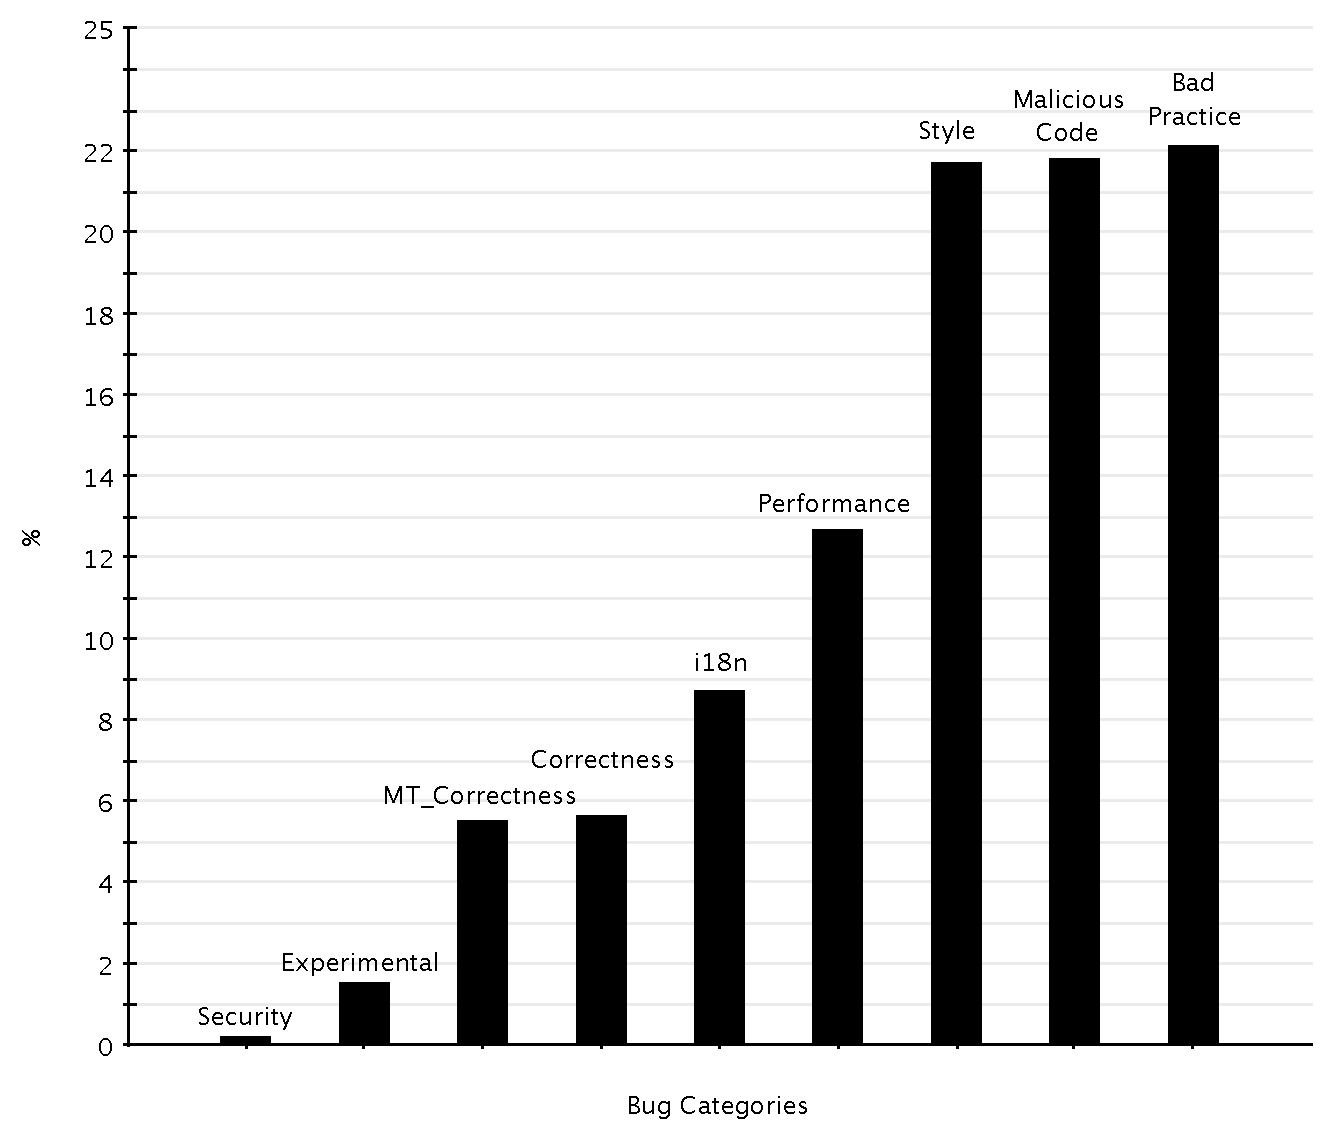
\includegraphics[scale=0.32]{figures/bug_percent}
	\caption{Bug percentage in Maven repository.}
	\label{fig:bug-per} 
\end{figure}

%But apart from such simple observations
%create scripts that can help us capture correlations
%that could provide interesting findings. For instance,

\section{Harnessing Our Dataset}
\label{sec:exploit}

Since Mongo{\sc db} provides a rich query interface,
it was easy to create
simple scripts to find out
how software bugs are distributed among the
repository (see Figure~\ref{fig:bug-per}).

Furthermore, we have created a series of
scripts to exhibit how the dataset can be used
to capture correlations regarding
the evolution of software bugs.
First, based on the dataset we produced some metadata
that contained the number of
bugs per category in each project version. Based
on these metadata we estimated the relation between
bugs and time (see Table~\ref{tbl:bugsperversion}).
Specifically, we calculated the Spearman correlations between the defects
count and the ordinal version number across all projects.
The zero tendency that can be seen on Table~\ref{tbl:bugsperversion}
applies to all versions of all projects together.

\begin{table}[b]
    \centering
\scalebox{0.94}{
        
\begin{tabular}{lcc}
\hline \\
Category & Spearman Correlation & $p$-value \\ \hline 
Security & 0.04 & $< 0.05$\\
Malicious Code & 0.03 & $\ll 0.05$\\
Style & 0.03 & $\ll 0.05$\\
Correctness & 0.04 & $\ll 0.05$\\
Bad Practice & 0.03 & $\ll 0.05$\\
{\sc mt} Correctness & 0.09 & $\ll 0.05$\\
i18n & 0.06 & $\ll 0.05$\\
Performance & {\it (0.01) } & 0.07\\
Experimental & 0.09 & $\ll 0.05$\\
\hline \\
\end{tabular}

}
	\caption{Correlations between version and defects count.}
    \label{tbl:bugsperversion}
\end{table}

In addition, we explored the relation between defects
with the size of a project
version, measured by the size of its {\sc jar} file by carrying out
correlation tests between the size and the defect counts for each
project and version. The results can be seen in
Table~\ref{tbl:jarsizecorr}.

Table~\ref{tbl:corrplot} presents the pairwise correlations
between all bug categories. To establish these correlations,
we calculated the correlations between the number of
distinct bugs that appeared in a project throughout its lifetime.

\begin{table}[hbt]
    \centering
\scalebox{0.94}{
    
\begin{tabular}{lcc}
\hline \\
Category & Spearman Correlation & $p$-value \\ \hline 
Security & 0.19 & $\ll 0.05$\\
Malicious Code & 0.65 & $\ll 0.05$\\
Style & 0.68 & $\ll 0.05$\\
Correctness & 0.51 & $\ll 0.05$\\
Bad Practice & 0.67 & $\ll 0.05$\\
{\sc mt} Correctness & 0.51 & $\ll 0.05$\\
i18n & 0.53 & $\ll 0.05$\\
Performance & 0.63 & $\ll 0.05$\\
Experimental & 0.36 & $\ll 0.05$\\
\hline \\
\end{tabular}

}
    \caption{Correlations between {\sc jar} size and defects count.}
    \label{tbl:jarsizecorr}
\end{table}

\begin{table*}[hbt]
    \centering
\scalebox{0.86}{
    
\begin{tabular}{lccccccccc}
\hline
Security & 1.00 & 0.20 & 0.22 & 0.27 & 0.20 & 0.33 & 0.20 & 0.31 & 0.32\\
Malicious Code & 0.20 & 1.00 & 0.63 & 0.63 & 0.56 & 0.56 & 0.62 & 0.60 & 0.48\\
Style & 0.22 & 0.63 & 1.00 & 0.68 & 0.62 & 0.63 & 0.66 & 0.58 & 0.46\\
Bad Practice & 0.27 & 0.63 & 0.68 & 1.00 & 0.54 & 0.58 & 0.64 & 0.63 & 0.51\\
Correctness & 0.20 & 0.56 & 0.62 & 0.54 & 1.00 & 0.56 & 0.55 & 0.52 & 0.52\\
{\sc mt} Correctness & 0.33 & 0.56 & 0.63 & 0.58 & 0.56 & 1.00 & 0.56 & 0.56 & 0.49\\
Performance & 0.20 & 0.62 & 0.66 & 0.64 & 0.55 & 0.56 & 1.00 & 0.60 & 0.52\\
i18n & 0.31 & 0.60 & 0.58 & 0.63 & 0.52 & 0.56 & 0.60 & 1.00 & 0.60\\
Experimental & 0.32 & 0.48 & 0.46 & 0.51 & 0.52 & 0.49 & 0.52 & 0.60 & 1.00\\
\hline
\end{tabular}

}
    \caption{Correlations between bug categories.}
    \label{tbl:corrplot}
\end{table*}

%\begin{figure}
%  \centering
%  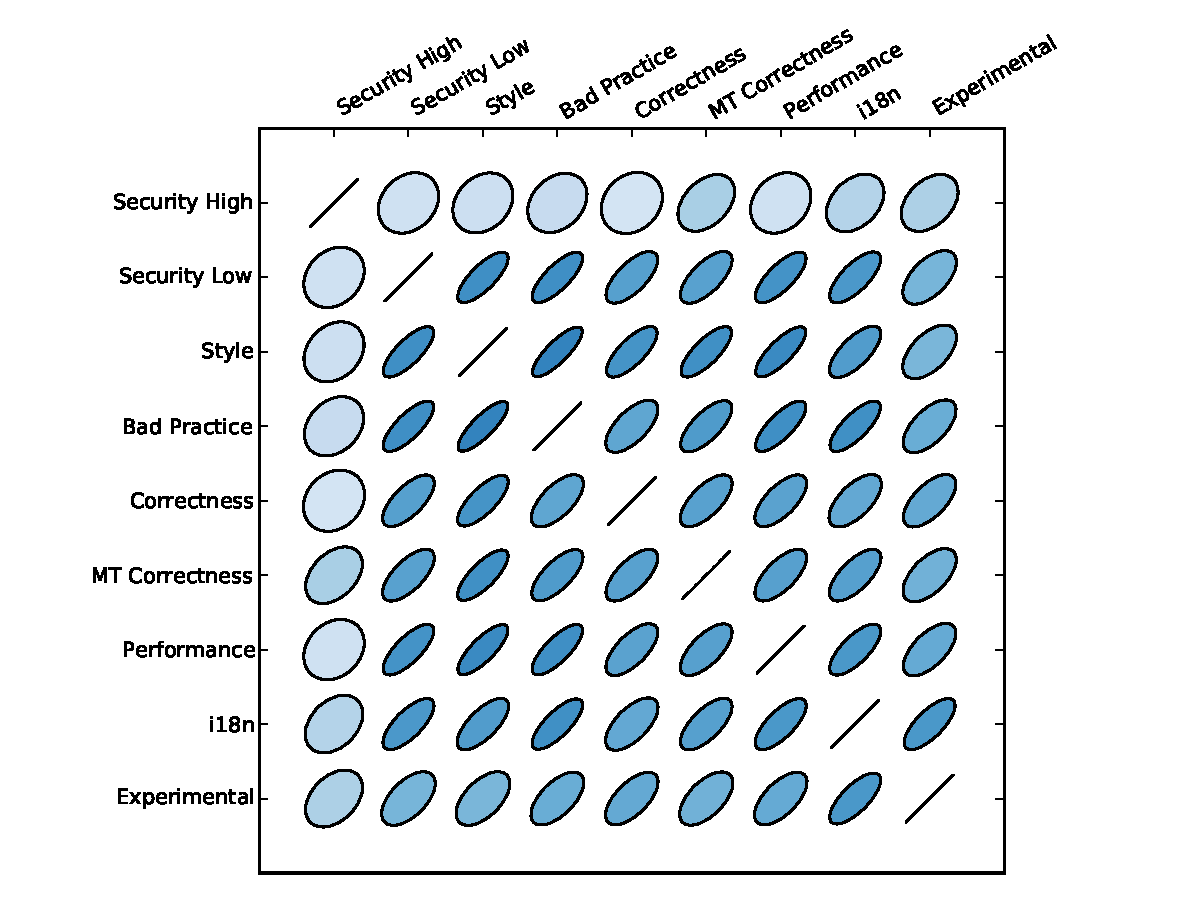
\includegraphics[scale=0.43]{corrplot.pdf}
%  \caption{Correlation matrix plot for bug categories.
%Blue color indicates positive correlation.
%The darker the color (and the more acute the ellipsis slant),
%the stronger the correlation.}
%  \label{fig:corrplot}
%\end{figure}

Research concerning the examination of specific bugs
can also be facilitated by our dataset. For instance,
we have examined the characteristics of security
bugs in a previous paper~\cite{MKLGS13}
based on this dataset.

\section{Limitations}
\label{sec:limit}

Limitations concerning out dataset involve some
{\sc jar}s that were in the initial {\sc jar} list
created during data cleaning but when the
FindBugs result collection was performed, they
were not online.

A threat to the internal validity of our dataset
construction process could be the false
alarms of the FindBugs tool~\cite{AP10}.
Specifically, reported security bugs may not
be applicable to an application's typical use context.
For instance, FindBugs could report an {\sc sql}
injection vulnerability
in an application that receives no external input.
In this particular context, this would be a false
positive alarm.

A disadvantage of our dataset is that as projects evolve
the dataset gets older. Also, even if we checked for
new project versions that could have been added
to the repository after the data cleaning and before
the results collection, we did not checked for new
projects added during this time frame.

\section{Related Work}
\label{sec:rel}

The Maven ecosystem has been previously analyzed by
Raemaekers et al.~\cite{RDV13}
to produce the {\it Maven dependency dataset}.
Apart from basic information like individual methods, classes,
packages and lines of code for every {\sc jar}, this dataset
also includes a database with all the
connections between the aforementioned elements.
Our work differs from this research because it
reports all bugs coming from the output of a
static analysis tool, for each {\sc jar}
contained in the Maven repository.

\section{Conclusions}
\label{sec:conc}

In this paper, we have presented a dataset that contains
for every {\sc jar} of the Maven central repository,
all the software bugs that it contains among with some
other metadata mentioned in Section~\ref{sec:exploit}.
We have also shown how our data can be
used to extract results concerning software evolution.

Note that our data collection process can be duplicated
in order to collect metrics results from other tools that
examine Java programs like
{\sc cjkm}\footnote{\small \url{http://www.spinellis.gr/sw/ckjm/}}
that calculates Chidamber and Kemerer
object-oriented metrics~\cite{CK91},
{\it Java Pathfinder}\footnote{\small \url{http://babelfish.arc.nasa.gov/trac/jpf/wiki}}
that performs
model checking~\cite{CEES09} on Java bytecode programs,
and others. To achieve this, instead of invoking
FindBugs, our worker can invoke such tools.

The complete set of our data and source code can be found at
\url{https://github.com/bkarak/data_paper_msr2014}.

\section{Acknowledgments}
This research has been co-financed by the
European Union (European Social Fund---{\sc esf}) 
and Greek national funds through the Operational
Program ``Education and Lifelong Learning" of the
National Strategic Reference Framework
({\sc nsrf})---Research Funding Program: 
Thalis---Athens University of Economics and
Business---Software Engineering Research Platform.

\bibliographystyle{abbrv}
\bibliography{msr}  

\end{document}
